\chapter{認識榮耀的基督（1:1-1:11）}

你在四福音書中所認識的耶穌，是怎樣的一位耶穌呢？
那是祂第一次來到地上。祂謙卑地來到我們中間，祂服事人，醫治病患，尋找失喪的人，祂並且「捨命作多人的贖價」。
許多天主教堂裡的耶穌形象，是釘在十字架上的耶穌。祂頭戴荊棘的冠冕，身上滿是鞭傷。祂是受苦、受死的耶穌。我們很難與想像中的「榮耀」聯繫在一起。

這是什麼原因呢？使徒保羅告訴我們，原來祂是本有神榮耀的形像的，可是他「卻虛己，取了奴僕的形像，存心順服，以至於死，且死在十字架上。」（腓立比書2:6–8）

但故事並沒有停在十字架上。「神將他升為至高，又賜給他那超乎萬名之上的名，叫一切在天上的、地上的、和地底下的，因耶穌的名，無不屈膝。」（腓立比書2:9-10）
這正是啟示錄要我們看見的榮耀的基督。

啟示錄一開始，就是榮耀的基督說話。

\begin{ScriptureBox2}{圈出1:4–8中所有用來稱呼耶穌基督的名字和稱號。1:3向念這預言、聽見並遵守的人應許了什麼？}

\item[1:1] 耶穌基督的啟示、就是　神賜給他、叫他將必要快成的事指示他的眾僕人．他就差遣使者、曉諭他的僕人約翰．

\item[1:2] 約翰便將　神的道、和耶穌基督的見證、凡自己所看見的、都證明出來。

\item[1:3] 念這書上預言的、和那些聽見又遵守其中所記載的、都是有福的．因為日期近了。

\item[1:4] 約翰寫信給亞西亞的七個教會．但願從那昔在今在以後永在的　神．和他寶座前的七靈．

\item[1:5] 並那誠實作見證的、從死裡首先復活、為世上君王元首的耶穌基督．有恩惠平安歸與你們。他愛我們、用自己的血使我們脫離罪惡．〔脫離有古卷作洗去〕

\item[1:6] 又使我們成為國民、作他父　神的祭司．但願榮耀權能歸給他、直到永永遠遠。阿們。

\item[1:7] 看哪、他駕雲降臨．眾目要看見他、連刺他的人也要看見他．地上的萬族都要因他哀哭。這話是真實的。阿們。

\item[1:8] 主　神說、我是阿拉法、我是俄梅戛、〔阿拉法俄梅戛乃希臘字母首末二字〕是昔在今在以後永在的全能者。

\item[1:9] 我約翰就是你們的弟兄、和你們在耶穌的患難、國度、忍耐裡一同有分．為　神的道、並為給耶穌作的見證、曾在那名叫拔摩的海島上。

\item[1:10] 當主日我被聖靈感動、聽見在我後面有大聲音如吹號說、

\item[1:11] 你所看見的、當寫在書上、達與以弗所、士每拿、別迦摩、推雅推喇、撒狄、非拉鐵非、老底嘉、那七個教會。

\end{ScriptureBox2}

\begin{ReaderQuestion}
如果我們知道將來要與基督一同作王、在神面前事奉，今天應當如何活出屬祂的身分？
\end{ReaderQuestion}

\section{啟示錄是約翰在拔摩島上記的}

約翰寫了約翰福音、約翰一書、約翰二書和約翰三書。
後來約翰在羅馬皇帝統治期間，因為基督信仰和為基督作見證而被放逐到拔摩海島。在島上記載了這卷啟示錄。
見圖\ref{fig:turkey-seven-churches}：
\ding{172}以弗所、\ding{173}士每拿、\ding{174}別迦摩、\ding{175}推雅推喇、\ding{176}撒狄、\ding{177}非拉鐵非、\ding{178}老底嘉。圈＝拔摩島。

\begin{figure}[htbp]
    \centering
    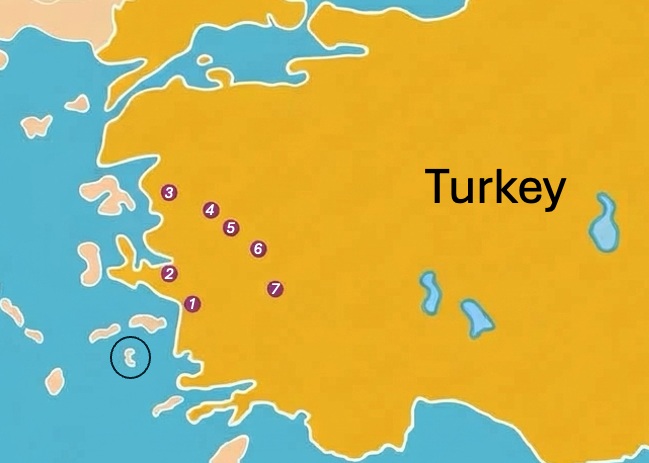
\includegraphics[
        width=0.9\textwidth,
        trim=0 0 0 100,
        clip
    ]{images/turkey}
    \caption{啟示錄七個教會的位置}
    \label{fig:turkey-seven-churches}
\end{figure}

在那孤獨、患難的環境中，他所看見的這些異象，會不會只是他的幻覺？
不是的。原因有二。第一，約翰並不是失去意識下而寫的。當異象出現時，他常常知道自己正在看見什麼，也記錄了天使對他的解釋。他甚至提出問題，並得到回答。
第二，啟示錄也是可靠的紀錄。第二世紀的教父愛任紐（Irenaeus）在《駁異端》（Against Heresies）中多次引用啟示錄。\footnote{
Irenaeus. (1885). \textit{Against heresies} (A. Roberts \& W. H. Rambaut, Trans.). Christian Literature Publishing. (Original work published ca. 180)}
愛任紐距離使徒約翰的時代並不遠。
到了第四世紀，史學家優西比烏（Eusebius）在《教會史》中整理早期教會傳統。他記載了約翰、拔摩以及圖密善時期的相關傳統。\footnote{
Eusebius. (1890). \textit{Church history} (A. C. McGiffert, Trans.).
Christian Literature Company. (Original work published ca. 325)}
優西比烏記載，約翰後來回到以弗所。\footnote{Eusebius, ca. 325/1885, 3.18.1, 3.20.9}
所以啟示錄是第一世紀真實流傳、保存並傳承的使徒見證。

啟示錄中的基督，是怎樣的基督呢？

\section{啟示錄中的榮耀基督}

如果你心中的耶穌是受苦的僕人，你更可以確定，祂原來是尊貴的君王。
新約歌羅西書 1:15 說「愛子是那不能看見之神的像」。希伯來書 1:3 也說「他是神榮耀所發的光輝，是神本體的真像」。
在啟示錄第一章到第三章中，我們看到許多關於耶穌的榮耀的描述。我們可以綜合成為表\ref{tab:christ-revelation-1-3}。

%\ref{fig:john_saw_christ_white.jpg}

{
\setstretch{1.0}
\begin{longtable}{p{1.6cm} p{7.3cm}}
\caption{啟示錄一至三章中對基督的形容}
\label{tab:christ-revelation-1-3} \\
\toprule
\textbf{經文} & \textbf{耶穌基督的形容} \\
\midrule
\endfirsthead

\toprule
\textbf{經文} & \textbf{耶穌基督的形容} \\
\midrule
\endhead

\bottomrule
\endfoot

\bottomrule
\endlastfoot

1:5
& 從死裡首先復活 \\
\midrule[0.2pt]
3:14
& 祂在一切受造之上，並超越地上的君王。 \\
\midrule[0.2pt]
1:8
& 祂是初，也是終；祂超越時間，掌管歷史。 \\
\midrule[0.2pt]
1:13
& 祂是真正的人類中的一位。祂身穿長衣，直垂到腳，胸間束著金帶。顯出祂尊貴、君王與祭司的身分。 \\
\midrule[0.2pt]
1:14
& 頭與髮皆白，如白羊毛，如雪。象徵聖潔與尊貴。是但以理書中的「亙古常在者」。 \\
\midrule[0.2pt]
1:14; 2:18
& 眼目如同火焰。祂洞察人心，察驗人的內心，無一事能在祂面前隱藏。 \\
\midrule[0.2pt]
1:15; 2:18
& 腳好像在爐中鍛鍊光明的銅；腳像光明銅的。象徵力量、純潔與公義的審判。 \\
\midrule[0.2pt]
1:15
& 聲音如同眾水的聲音，帶著威嚴與權柄。 \\
\midrule[0.2pt]
1:16; 2:1; 3:1
& 右手拿著七星；在七個金燈臺中間行走；有神的七靈和七星的。祂掌管教會，也在教會中間行走、察看，並掌管聖靈的工作。 \\
\midrule[0.2pt]
1:16; 2:12
& 從祂口中出來一把兩刃的利劍；那有兩刃利劍的。祂以真理審判錯謬與罪惡，也以祂的話語勝過仇敵。 \\
\midrule[0.2pt]
1:16
& 面貌如同烈日放光。顯明祂的尊貴與神聖。 \\
\midrule[0.2pt]
1:18
& 拿著死亡和陰間的鑰匙。 \\
\midrule[0.2pt]
3:7
& 拿著大衛的鑰匙。祂擁有大衛君王的權柄，開了就沒有人能關。 \\
\midrule[0.2pt]
3:14
& 誠信真實見證的。祂是完全可靠、真實的見證。 \\
\end{longtable}
}

\begin{ReaderQuestion}
在表\ref{tab:christ-revelation-1-3}中，圈出那些與你平常心中耶穌形象不同的字詞。這表中的基督，與你心中的形象有什麼不同？
\end{ReaderQuestion}

\section{舊約早已預告基督的榮耀}
\label{sec:ch01_ot}

而且，約翰所描述的榮耀基督，與舊約先知在數百年前所看見的異象非常相似。
這不是巧合。熟讀舊約的猶太人讀到啟示錄中的基督，就會認出祂正是舊約所預告、所盼望的那位榮耀君王。
\begin{itemize}
\item 但以理書7:9：「我觀看、見有寶座設立、上頭坐著亙古常在者、他的衣服潔白如雪、頭髮如純淨的羊毛、寶座乃火焰、其輪乃烈火．」
\item 但以理書7:13：「我在夜間的異象中觀看、見有一位像人子的、駕著天雲而來、被領到亙古常在者面前。」
\item 但以理書7:14：「得了權柄、榮耀、國度、使各方各國各族的人都事奉他．他的權柄是永遠的、不能廢去、他的國必不敗壞。」
\item 但以理書10:6：「他身體如水蒼玉、面貌如閃電、眼目如火把、手和腳如光明的銅、說話的聲音如大眾的聲音。」
\item 以西結書43:2：「以色列　神的榮光從東而來．他的聲音如同多水的聲音．地就因他的榮耀發光。」
\item 以賽亞書22:22：「我必將大衛家的鑰匙放在他肩頭上．他開、無人能關．他關、無人能開。」
\end{itemize}
這些先知都曾在艱難的時代中看見基督的榮耀。榮耀的主沒有忘記祂的僕人，反而向他們顯明自己的榮耀，成為他們的力量和盼望。

如果你心中的耶穌只有受苦、被棄絕、被釘十字架的一面，那麼你需要再次提醒自己：祂本有神的形象，也是已經復活、得勝、掌權的榮耀之主。

\begin{ReaderQuestion}
同一位基督曾取了奴僕的形象、為我們受苦、被棄絕並死在十字架上，如今卻坐在寶座上、掌管列國。這兩個面向如何幫助我們更完整地認識耶穌？
\end{ReaderQuestion}

因此，當我們認識這位榮耀的基督，就能在今天的苦難中仍然有盼望，在軟弱中仍然有力量，在黑暗中仍然忠心，直到祂再來。

\begin{ReaderQuestion}
當教會面對患難、逼迫、試探與軟弱時，認識基督是首先的、末後的、曾死過又活著、並且拿著死亡和陰間的鑰匙，如何幫助我們仍然忠心持守？
\end{ReaderQuestion}
